\documentclass[a4paper,11pt,titlepage,uplatex]{jsarticle}

% プリアンブルを外部ファイル化しておきました。中身はmacro.texで確認できます。

\usepackage[dvipdfmx]{graphicx,xcolor}% ドライバ指定
\usepackage[top=30truemm,bottom=30truemm,left=25truemm,right=25truemm]{geometry} % 余白設定

% 画像
\usepackage{here, subfig}
\usepackage{docmute} % ファイル分割用
\usepackage[cc]{titlepic}

% 数式関連
\usepackage{amsmath,amsfonts,amssymb,mathtools,amsthm}
\usepackage{bm} % ボールド体のベクトルを出力するときには\vb{a}ではなく\bm{a}としてください。\bmの方が綺麗に出力できる。
\usepackage{empheq} % 連立方程式をきれいに書いてくれる
\usepackage{physics} % 微分記号とか
\usepackage[separate-uncertainty]{siunitx} % SIUNITX

% 数式、図、表番号の変更
\makeatletter
\@addtoreset{equation}{section} % 章ごとに番号をリセット
\@addtoreset{figure}{section}
\@addtoreset{table}{section}
\def\theequation{\thesection.\arabic{equation}} % 章.何番目 と変更
\def\thefigure{\thesection.\arabic{figure}}
\def\thetable{\thesection.\arabic{table}}
\makeatother

% -------------------
% 定理環境付近
\usepackage{tcolorbox} % 色付きの囲み
\tcbuselibrary{breakable, skins, theorems}
\usepackage{ascmac} % 囲み \begin{itembox}ができる。

% ----------

\usepackage{enumitem} % enumium環境いじるために必要
\renewcommand{\labelenumi}{\theenumi.}
\renewcommand{\theenumi}{\Alph{enumi}}

% ------------ url関係
\usepackage{url}
\usepackage[dvipdfmx]{hyperref}
\hypersetup{
	 colorlinks=true,
	 citecolor=blue,
	 linkcolor=black,
	 urlcolor=blue
}
\usepackage{pxjahyper}
% ---------

% 表関連のパッケージ
\usepackage{booktabs}
\usepackage{multirow}
\usepackage{longtable}
\usepackage{arydshln}% 表で破線を使うため
\usepackage{multicol}
% longtableをusepackageする場合は順番が重要らしいです。longtableとarydshlnの順番逆にしたらエラーはく(コンパイルはできるが…)

\renewcommand{\labelitemii}{・}

\usepackage[greek, japanese]{babel}
\usepackage{teubner}	% 古代(古典)ギリシア語表記指定



% 大槻使用
\usepackage{color}
\newcommand{\red}[1]{\textcolor{red}{#1}}
\newcommand{\blue}[1]{\textcolor{blue}{#1}}
\usepackage{ulem}

% 能崎使用
%背景
\usepackage{wallpaper}

\begin{document}

\section{プロジェクト概要}
本プロジェクトは、団体初の動翼機構をC-59Jに搭載し、ロール制御を行うことを目的としたプロジェクトである。
機体に搭載したピトー管により、飛翔時の対気速度をリアルタイムで取得した。対気速度によって変化するロールモーメントの大きさを考慮しながら、ロール角度に関するフィードバック制御を行うことを目指した。
本プロジェクトの目的は、ロケットのロール制御技術を獲得・実証し、姿勢制御技術の足掛かりを得ることである。

\subsection{ミッション目標}
本プロジェクトのミッション目標は以下の通りである:
\begin{itemize}
    \item ピトー管によって対気速度をリアルタイムで取得する。
    \item 燃焼停止からパラシュート開傘までのロール制御を行う。
\end{itemize}

1番のミッション目標は機体のロール制御を行うことである。ところで、ロール制御の精度を上げるためには対気速度をリアルタイムで取得する必要があり、
その方法の1つとしてピトー管を搭載することが挙げられる。
しかし、現在のCREATEにはピトー管の作成・評価技術が存在していないため、第18回能代宇宙イベント\footnote{2022年8月11日から2022年8月19日まで行われた、秋田県能代市を会場とした宇宙イベントである。\\
    能代宇宙イベント公式ホームページ:\url{http://www.noshiro-space-event.org/}}
においてC-61J\footnote{第21回伊豆大島共同打上実験にてCREATEが打ち上げた2021年度新入生機体である。}がC-59Jに先行してピトー管を搭載し、技術検証をする予定であった。
しかし、C-59Jと同じ第21回伊豆大島共同打上実験での打上げとなったため、ピトー管の技術検証もC-59Jのミッション目標に含まれることになった。なお、サクセスクライテリアについてはロール制御ミッションのみに設定してある。
% \footnote{後に述べるように、事前の風洞実験においてもピトー管の精度を担保することができなかったため、ピトー管による精度の影響を受けにくい制御を行った。}

\subsection{ミッション背景}
次に、ミッション背景について述べる。CREATEのロケットはロール運動しながら飛行していることが以前の打上実験から判明している。
本来ならばロール運動をしないような構造設計をしているため、ロール運動をしながら飛翔することは好ましくない。
特に2段式技術実証機であるC-43Jプロジェクトにおいて、機体の姿勢角条件が2段目分離条件を満たしておらず、電装部の安全機構により2段目が放出されなかった。
以上の結果より、機体の姿勢制御技術を発展させ、より安定した飛翔を目指すことが団体の課題であった。

また、ピッチ・ヨー制御と比較してロール制御を行うメリットとして、制御による飛行経路の影響が少ないということが挙げられる。
これは、ロール回転運動がピッチ・ヨー回転運動に影響を与えないことに基づいている。
機体が予想外のピッチ・ヨー回転運動をする場合、機体の飛行経路に大きな影響を与えることが知られている。
すなわち、ピッチ・ヨー制御を行うことはロール制御よりも安全面から困難であると考えた。
そのため、C-59Jでは姿勢制御技術の発展の第一歩としてロール制御をミッションとした。

\newpage
\subsection{サクセスクライテリアについて}
以下の表\ref{tab:success_criteria}に本プロジェクトのサクセスクライテリアを示す。なお、FULLのサクセスクライテリアについては表とは別に詳述する。
\begin{table}[H]
    \centering
    \caption{サクセスクライテリア}
    \begin{tabular}{cp{60mm}p{60mm}} \toprule
             & \multicolumn{1}{c}{内容}                                   & \multicolumn{1}{c}{判定条件}             \\ \midrule
        MIN  & 地上で制御プログラムを実行し、動翼の適切な動作を確認する。                            & 動画とデータ解析により、意図した動翼の動作が実現していることを確認する。 \\ \midrule
        FULL & ロール制御を成功させる。                                             & 搭載カメラの映像とデータ解析によって確認する。              \\ \midrule
        ADV  & 制御前に機体がロールをしていた場合、制御中は目標角からのロール角度を\SI{90}{\degree}以下にする。 & データ解析で内容を達成しているか確認する。                \\
        \bottomrule
    \end{tabular}
    \label{tab:success_criteria}
\end{table}
\subsubsection*{FULLのサクセスクライテリアについて}
FULLのサクセスクライテリアの意味としてのロール制御の成功条件を述べる。まずは以下に文Aと文Bを示す:
\begin{enumerate}
    \item ある程度一定方向を向き続けた映像が撮れている。
    \item 意図したロール制御が実現されている。
\end{enumerate}

FULLのサクセスクライテリアでの意味としてロール制御が成功しているとは、文Aと文Bが同時に満たされている場合であると定義する。
次に、文Aと文Bをサクセスクライテリアの成功可否に用いる理由について述べる。
そもそもロール制御が成功しているとは、「ロール制御が何らかの結果として成功しており、実際にロール角度が一定に保たれていること」と、「ロール制御が制御系の正常な動作によって引き起こされたものであること」を同時に満たしている状況のことである。
ここで文Aは、ロール角度が一定に保たれていることを定性的に確認するために導入した。制御に関する電装データを取得すれば良いかもしれないが、そのデータが間違っている可能性を排除する必要がある。
すなわち、C-59Jの機体動翼部に搭載しているカメラ映像や6軸センサでのロール角の値を用いることで、制御部に依らず独立に確認できる条件とした。
そして文Bは、ロール角度が一定に保たれているかとは独立に、制御系の正常な動作を定量的に確認するために導入した。

文Aの達成可否については機体に搭載したカメラによって判定する。ロール制御が成功している場合には、カメラ映像でロール角度が一定に保たれていることが目視で判別することができる。
次に、文Bの達成可否については電装データによって定量的に判定する。先に述べたように、カメラ映像によってロール制御が成功していると判断できても、制御系が正常に機能していることの確認にはならない。
すなわち、カメラの映像で定性的にロール制御の成功を確認するだけでなく、それが意図した制御によって実現されたことを確認する必要がある。
したがって、ロール角度や動翼角度のログデータ、実際の制御系の応答、目標角度の追従率などから定量的に成功可否を判断する。

\newpage
\subsection{機体ロゴ}
C-59J(愛称:IRIS)の機体ロゴを以下の図\ref{fig:sum_kitairogo}に示す。
\begin{figure}[H]
    \centering
    
\includegraphics[width=0.5\linewidth]{pic_summary/newlogo.png}
    \caption{機体ロゴ}
    \label{fig:sum_kitairogo}
\end{figure}
ロゴデザインのモチーフは、C-59Jの愛称である``IRIS''からきている。
IRISはギリシャ神話に登場する虹の女神IRIS (\foreignlanguage{greek}{{>~I}ris})から取られており、機体に虹が架かる様子を表している。



\section{C-59J開発概要}
本章では、C-59Jの開発概要について簡単に説明する。詳細な開発内容については次章以降に示す。
\subsection{設計思想}
\subsubsection{ミッション・シーケンス}
本ミッションのミッション・シーケンスを以下に示す。なお、$\mathrm{X}$は打上時刻($\mathrm{X}$時刻)を表している。
\begin{enumerate}
    \renewcommand{\labelenumi}{\arabic{enumi}.}
    \item $\mathrm{X}+0$でハイブリットエンジンに点火する。
    \item 燃焼終了直後から動翼機構によるロール制御を開始する。
    \item 頂点検知後にパラシュートを展開し降下する。
\end{enumerate}


電装の概要を図\ref{fig:avi_all}に示す。
\begin{figure}[H]
    \centering
    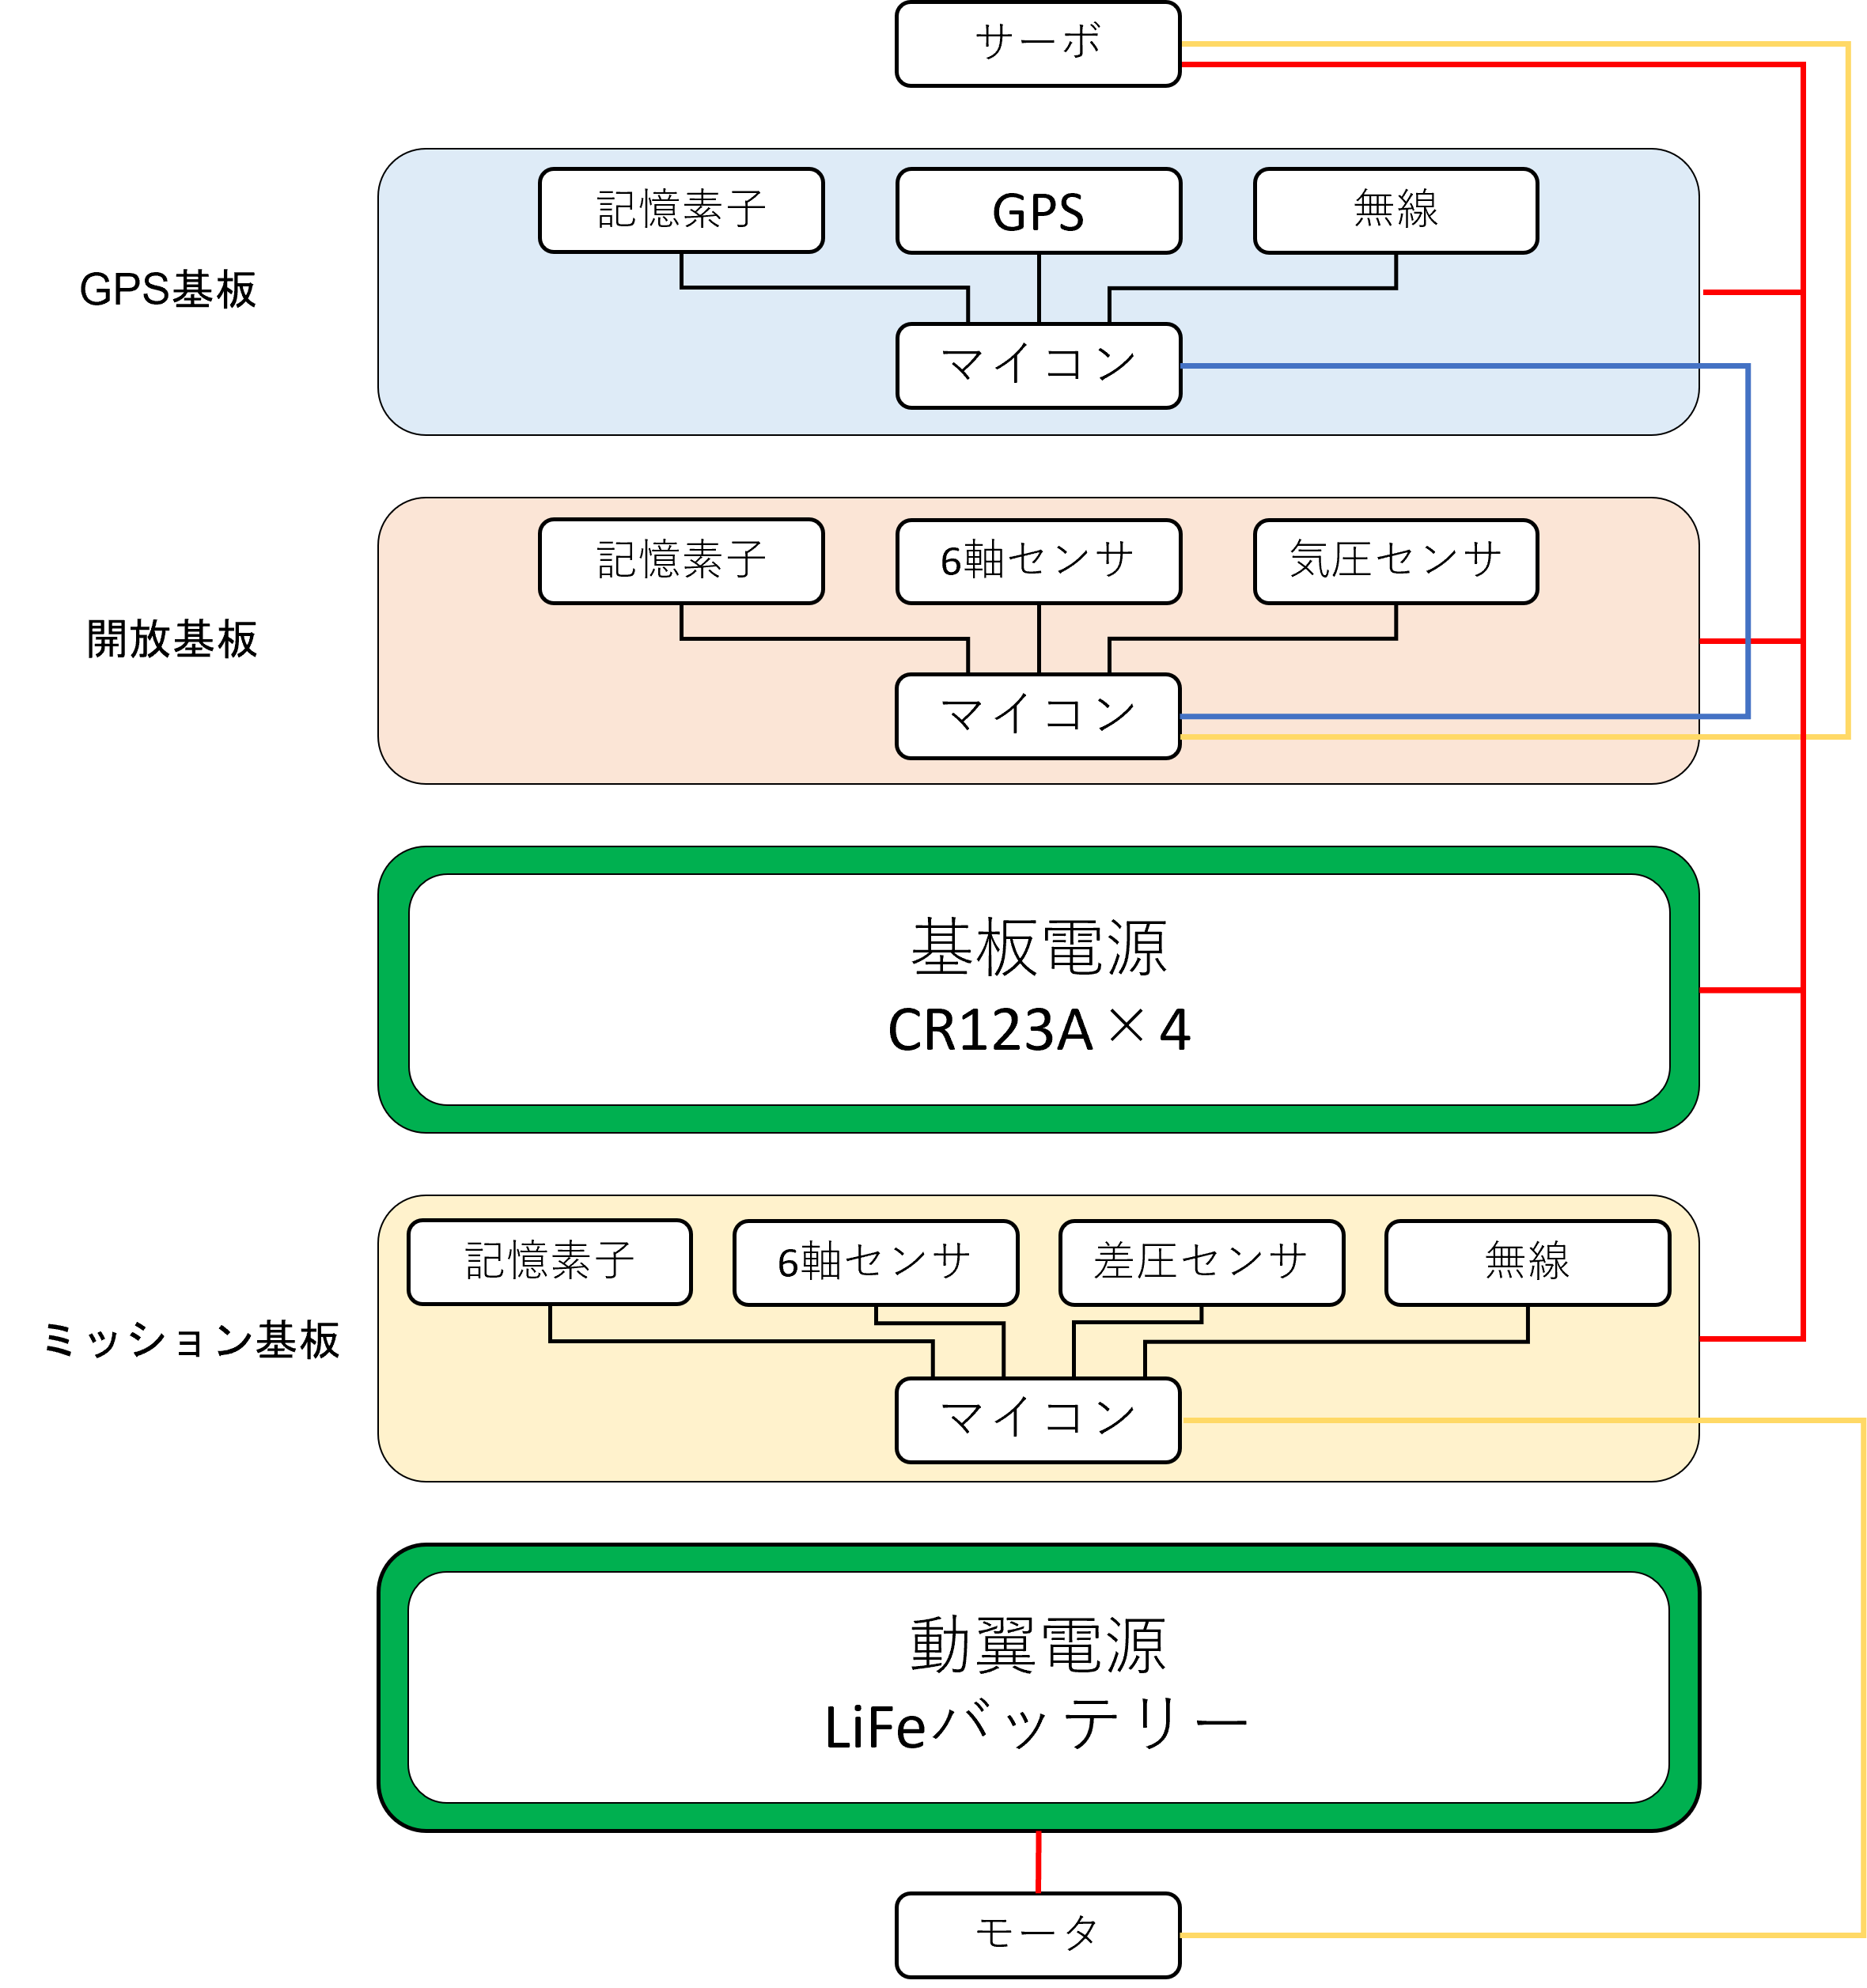
\includegraphics[width=0.8\linewidth]{pic_summary/avi_all.png}
    \caption{電装概要}
    \label{fig:avi_all}
\end{figure}

基板ごとの役割を表\ref{tab:avi_ref}に示す。
\begin{table}[H]
    \centering
    \caption{基板ごとの役割}
    \begin{tabular}{cccc} \toprule
        基板      & 役割         \\ \midrule
        GPS基板   & GPSのダウンリンク \\
        開放基板    & 減速機構の制御    \\
        ミッション基板 & 動翼の制御      \\
        \bottomrule
    \end{tabular}
    \label{tab:avi_ref}
\end{table}

\end{document}